\documentclass[UTF8]{ctexart}
\usepackage{amsmath}
\usepackage{amssymb}
\usepackage{booktabs}
\usepackage{background}
\usepackage{caption,subcaption}
\usepackage{enumitem}
\usepackage{fancyhdr}
\usepackage{float}
\usepackage{fontspec}
%\usepackage{fourier}
\usepackage{geometry}
\usepackage{imakeidx}
\usepackage{listings}
\usepackage{pifont}
\usepackage{tcolorbox}
\tcbuselibrary{breakable}
\usepackage{tikz}
\usetikzlibrary{arrows.meta, positioning, shapes.geometric, calc}
\usepackage{xcolor}

\geometry{a5paper, top=0.1cm, left=1cm, right=1cm, bottom=1cm, footskip=0.1cm}
\setCJKmainfont[BoldFont={汉仪文黑-85W},ItalicFont={方正苏新诗柳楷简体}]{汉仪文黑-55W}
\setfontfamily\Issue{Century Schoolbook}
\setfontfamily\Genshin{Genshin Teyvat Lingua Franca}
\newCJKfontfamily\TitleFont{思源宋体 CN Heavy}
\newfontfamily\timesnewroman{Times New Roman}
\captionsetup{font=small, labelfont=bf}

\pagestyle{fancy}
\fancyhf{}
\cfoot{\sffamily\footnotesize{-\ \thepage\ -}}
\CTEXsetup[format={\bfseries\large}]{paragraph}
%\CTEXsetup[format = {\centering\bfseries\large}, beforeskip = 3pt, afterskip = 3pt]{section}

\colorlet{darkcyan}{cyan!50!black}
\newcommand\Black[1]{\textcolor[gray]{0.3}{#1}}
\newcommand\Brown[1]{\textcolor[HTML]{998A4E}{#1}}
\newcommand\Emph[1]{\colorbox{green!10}{\textcolor{green!30!black}{#1}}}
\newcommand\Notes[1]{\textcolor{yellow!50!black}{\small #1}}
\newcommand\Example[1]{\textcolor{cyan!70!black}{\small #1}}


\lstset{
    basicstyle=\small\ttfamily, %注意行末有逗号!
    keywordstyle=\bfseries\color{blue!70!black},
    commentstyle=\color{cyan!90!black},
    stringstyle=\color{green!40!black},
    columns=flexible,
    numbers=left,
    numberstyle=\footnotesize,
    escapechar=`,
    frame=shadowbox,
    %rulesepcolor=\color{red!20!blue!20!green!20}
    backgroundcolor=\color{cyan!5!white},
    language = SQL,
    tabsize = 4,
    breaklines = true,
}

% -----------------本文档专用-----------------
\newcommand\Rare[1]{\colorbox{cyan!30}{\textcolor{cyan!40!black}{\bfseries #1}} \index{#1} }
\newcommand\Epic[1]{\colorbox{violet!15}{\textcolor{violet}{\bfseries #1}} \index{#1}}
\newcommand\Legend[1]{\colorbox{orange!30}{\textcolor{orange!60!black}{\bfseries #1}} \index{#1}}

\newtcolorbox{summaryBox}[1][本章要求]{colback=green!10, colframe=green!60!black, arc=1mm, title={#1}, breakable}
\newtcolorbox{subject}[1]{colback=teal!10, colframe=teal, arc=1mm, boxrule=1pt, fonttitle=\bfseries, fontupper=\small, title={#1}}

\makeindex[columns=2, title={名词索引}, columnseprule] % 索引格式
% ---------------------------------------------

\newcommand\IssueNumber{53}
\newcommand\Date{2025-4-23}
%\newcommand\Contributer{@金光日}
\newcommand\Subject{计算机系统结构}
%\newcommand\Source{2023 考研 408 真题}


\begin{document}
\backgroundsetup{contents=
\includegraphics{上半示例.png}, center, scale=1, angle=0, opacity=1}
\BgThispage
\begin{center}
%{\scriptsize\Issue \textcolor[HTML]{C8BA83}{\Genshin WEEKLY TIPS}}
\phantom{...}

{\Large\textcolor{brown!40!white}{\makebox[10cm][s]{\Genshin WEEKLY KNOWLEDGE TIPS}}}

\vspace{-2em}

{\Huge\bfseries\TitleFont \Black{知\ 识\ 小\ 料}}


\vspace{-0.1cm}
{\footnotesize \Brown{「电计 2203 班」周常规知识整理共享}}
\end{center}

\vspace{-0.5cm}


\begin{figure}[H]
\hspace{1cm}
\begin{minipage}[t]{0.3\textwidth}
\centering
    \Brown{\Genshin ISSUE}

    \vspace{-0.6cm}
    \Huge \Issue\slshape\bfseries\Black{\IssueNumber}
\end{minipage}
\hfill
\begin{minipage}[t]{0.35\textwidth}
\centering
    \Brown{日期:\Date} \\
%\vspace{-0.1cm}
%    \Brown{贡献者:\Contributer} \\
\vspace{-0.1cm}
    \Brown{学科:\Subject} \\
%\vspace{-0.1cm}
%    \Brown{来源:\Source} \\
\end{minipage}
\hspace{0.8cm}
\end{figure}

{\centering\color{darkcyan}本文档对《计算机系统结构》(Computer Architecture)课程作出简明复习。}

\begin{quote}\small
\begin{center}
    \bfseries 说\quad 明
\end{center}

本文档采用以下方式标识概念/知识点重点等级,星级越高表示概念/知识点越重要。整理基于作者本人看法,请以实际为准。示例如下:
\begin{itemize}
    \item \colorbox{cyan!30}{\textcolor{cyan!40!black}{\bfseries 记分板算法}}:\textcolor{cyan!40!black}{稀有(\ding{72}\ding{72}\ding{72})}概念,要求了解;
    \item \colorbox{violet!15}{\textcolor{violet}{\bfseries 转移历史表(BHT)}}:\textcolor{violet}{史诗(\ding{72}\ding{72}\ding{72}\ding{72})}概念,要求理解;
    \item \colorbox{orange!30}{\textcolor{orange!60!black}{\bfseries Amdahl定律}}:\textcolor{orange!60!black}{传说(\ding{72}\ding{72}\ding{72}\ding{72}\ding{72})}概念,要求重点掌握与运用。
\end{itemize}
\end{quote}

\tableofcontents %参数代表展开到第3级
\backgroundsetup{contents=
\includegraphics{空白示例.png}, center, scale=1, angle=0, opacity=1}
\BgThispage
\newpage

\section{(第 1 章) 计算机系统结构概述}

\subsection{何为「计算机体系/系统结构」}
\begin{itemize}
    \item 引子:按下PPT翻页原理
    \item \Epic{计算机层次结构}:最高层为应用程序,其次为操作系统,第三为硬件系统,最底层为硅片工艺。相邻两层之间各有充当「接口」的角色,依次为 API、ISA、工艺模型。
    \item \Rare{冯·诺依曼结构}:数据和程序都在存储器中,CPU从内存中取指令和数据进行运算,并把结果也放到内存中。
\end{itemize}

\subsection{衡量计算机的指标——性能、价格、功耗}

\subsubsection{性能} 计算性能常用到 CPI 这一定义。
\begin{itemize}
    \item \Legend{CPI}:Cycle Per Instruction,即每条指令所需要的时钟周期数。
\end{itemize}

\begin{subject}{专题·CPU 时间计算}
\begin{itemize}
    \item CPU 计算时间公式如下:
    \begin{equation}\label{eq:CPU-time}
        T_{\text{CPU}} = I_N\times CPI \times T_{\text{c}}
    \end{equation}
        \begin{itemize}
            \item $I_N$:指令条数
            \item $CPI$:每条指令的时钟周期数
            \item $T_{\text{c}}$:时钟周期
        \end{itemize}

    \item 若有多个 CPI,平均 CPI 以\textbf{使用频次}为权重作加权平均:$\overline{CPI} = \sum_{j=1}^n CPI_j\cdot F_j$,其中 $F_j=\dfrac{I_j}{I_N}$(第 $j$ 类指令指令数量占比)。

    \item 要计算增强后的 CPI,可以使用 \colorbox{teal!30}{$CPI_{\text{新}} = CPI_{\text{原}} - \Delta CPI$} 思路计算。
\end{itemize}
\end{subject}

\begin{itemize}
    \item \Rare{影响CPU性能的因素}:
    \begin{enumerate}
        \item 优化算法:影响 $I_N$
        \item 优化编译器:影响 $I_N,CPI$
        \item 优化指令集(ISA):影响 $I_N,CPI$
        \item 优化微结构:影响 $CPI,T_\mathrm{c}$
        \item 优化主频:影响 $T_\mathrm{c}$
    \end{enumerate}
    \item \Rare{计算机性能评价原则}:以基准测试程序为基准,个人机更关注响应时间,工作站更关注吞吐率。
    \item \Rare{基准测试程序}:用以评价计算机性能,常见的有 SPEC 系列程序。
\end{itemize}

\paragraph{成本、功耗} 也是衡量计算机的指标。

\subsection{系统结构发展趋势}
\begin{itemize}
    \item \Epic{摩尔定律}:晶体管数目每 18--24 个月翻一番;同样晶体管数量的芯片价格下降一半。摩尔定律的阻力的三个阶段的体现:
    \begin{enumerate}
        \item 晶体管不够用
        \item 存储器速度慢
        \item 晶体管过多而越发难用
    \end{enumerate}
    \item 系统结构发展之「墙」:存储墙、功耗墙;带宽墙、成本墙、应用墙……
\end{itemize}

\subsection{系统结构设计原则}
\begin{itemize}
    \item 系统结构设计的原则:平衡性、局部性、并行性、虚拟化。
    \item \Legend{Amdahl 定律}:计算机部分性能的提高,受制于其时间占比,类似「短板效应」。
\end{itemize}

\begin{subject}{专题·Amdahl计算题}
\begin{itemize}
    \item 增强比例 $F$:被改进部分的时间占比,取值 $[0\%, 100\%]$。
    \item 增强加速比 $S$:被改进部分改进后与改进前的性能提高倍数,取值大于 1。
\end{itemize}

\begin{equation}\label{eq:Amdahl}
    \text{增强后用时} T_\mathrm{new} = T_\mathrm{old}\times \left(\dfrac{1-F}{1}+\dfrac{F}{S}\right)
\end{equation}
\begin{equation}\label{eq:Amdahl-2}
    \text{总加速比} S_\mathrm{overall} = \dfrac{T_\mathrm{old}}{T_\mathrm{new}} = \dfrac{1}{\dfrac{1-F}{1}+\dfrac{F}{S}}
\end{equation}
理想情况下,$S\to\infty$ 时,最大的总加速比 $S_\mathrm{overall} = \dfrac{1}{1-F}$。
\end{subject}

\subsection{支线[L01.1]·计算机设计新趋势}
\begin{itemize}
    \item \Rare{Top500}是一个统计高性能计算机性能,并公布前 500 名计算机系统的网站。
    \item \Rare{神威·太湖之光} 是中国国内第一台全部采用国产处理器构建的世界第一的超级计算机,坐落于无锡,于 2022 年在 Top500 网站上斩获第六名。\textcolor{gray}{(如今中国最先进的计算机在 Top500 网站上不参评,韬光养晦。)}
    \item 国产 CPU 厂商有:龙芯、鲲鹏、申威、海光等。其中龙芯系列芯片是完全自主知识产权的国产芯片。
\end{itemize}

\section{(第 2 章)指令系统}
\subsection{指令系统}
\begin{itemize}
    \item \Epic{指令系统(ISA)} 是软硬件的交界面,承应用软件与系统软件,启硬件系统与电路器件。它反映了结构设计者对计算机系统的认识。
    \item 当前主流的两种指令系统为 x86 和 ARM,此外还有 RISC-V、MIPS 等。
    \item 指令系统的设计原则:兼容性、通用性、高效性、安全性。
\end{itemize}

\subsection{指令系统的演变}
\begin{itemize}
    \item 根据指令长度分类:CISC、RISC、VLIM
    \item \Rare{RISC 指令}:简化指令间关系,有利于指令流水线高效实现。采用 Load/Store 结构。
    \item 存储管理的演变:段式、页式、段页式。
    \item 运行级别的演变:调试模式、主机模式、客户机模式。
    \item 根据使用数据方式分类:堆栈型、累加器型、寄存器型。
\end{itemize}

\subsection{指令系统的组成}
\begin{itemize}
    \item \Rare{大端序}:指数据的高位放在地址的低位。规定网络字节序为大端序。
    \item \Rare{小端序}:指数据的低位放在地址的低位。
\end{itemize}

\begin{table}[htb]
    \centering
    \begin{tabular}{|c|c|c|c|c|}
        \hline
        地址 & 2000 & 2001 & 2002 & 2003 \\
        \hline
        大端序 & \verb!01! & \verb!23! & \verb!45! & \verb!67! \\
        \hline
        小端序 & \verb!67! & \verb!45! & \verb!23! & \verb!01! \\
        \hline
    \end{tabular}
    \caption{存放 int 型整数 \texttt{0x01234567}}\label{tab:Big-and-little-endian}
\end{table}

\begin{itemize}
    \item 寻址方式:支持寄存器寻址、存储器寻址、立即数寻址、比例寻址等。其中比例寻址用于按列访问。
    \item 指令操作:通常包括算术逻辑指令、访存指令、转移指令、系统指令。
    \item 指令编码:定长编码(RISC)、变长编码(x86,ARM)、混合编码(IBM,MIPS)。
    \item \textcolor{gray}{RISC指令系统比较:“亲兄弟”和“表兄弟”。}
    \item \textcolor{gray}{C语言的机器表示。}
\end{itemize}

\section{(第3章)特权指令系统与 ABI}
\begin{itemize}
    \item \Rare{特权指令系统}:指用户和编译器无法触及的那部分指令系统,只用于操作系统等系统软件。
    \item \Rare{应用程序二进制接口(ABI)}:是操作系统对应用程序在这个系统下运行时必须遵守的编程约定。
    \item \Rare{应用程序编程接口(API)}:是一组预先定义的函数或指令集,允许不同的软件应用程序之间进行交互和通信。\textcolor{gray}{(易混概念)}
\end{itemize}

\section{(第9章)指令流水线·上}
\subsection{支线[L09.0]·流水线基本概念}
\begin{itemize}
    \item 流水线的时空图
    \item 流水线的「通过时间」和「排空时间」
    \item 按反馈回路分:「线性流水线」和「非线性流水线」,前者只有串行连接,后者有反馈回路。
    \item 按功能分:「单功能流水线」和「多功能流水线」。其中多功能流水线进一步划分:
    \begin{enumerate}
        \item \Epic{静态多功能流水线}:静态流水线的不同的功能(如加法和乘法)不允许在同一时间片内同时出现,必须等一种功能的流水线全部排空才可以运行其他功能。
        \item \Epic{动态多功能流水线}:同一时间内,各段可以按照不同的方式连接,同时执行多种功能。允许指令乱序执行。
    \end{enumerate}
\end{itemize}

\subsection{流水线处理器}
\begin{itemize}
    \item CPU数据通路,包括 PC、指令存储器、译码部件、通用寄存器、ALU 等。在此基础上添加模块:
    \begin{enumerate}[itemsep=0pt,parsep=0pt]
        \item 控制逻辑:位于指令每一级的寄存器处
        \item 有效位标记:位于指令每一级的寄存器处
        \item 寄存器相关判断逻辑
        \item 前递机制
    \end{enumerate}
    \item \Epic{流水线冒险}、\Epic{指令相关}与\Epic{指令冲突},相关概念如下图 \ref{fig:pipeline-adventure} 所示。此外,相关性的存在只预示着存在有冲突的可能性,不代表一定产生冲突。
\end{itemize}

\begin{figure}[htb]
    \centering
    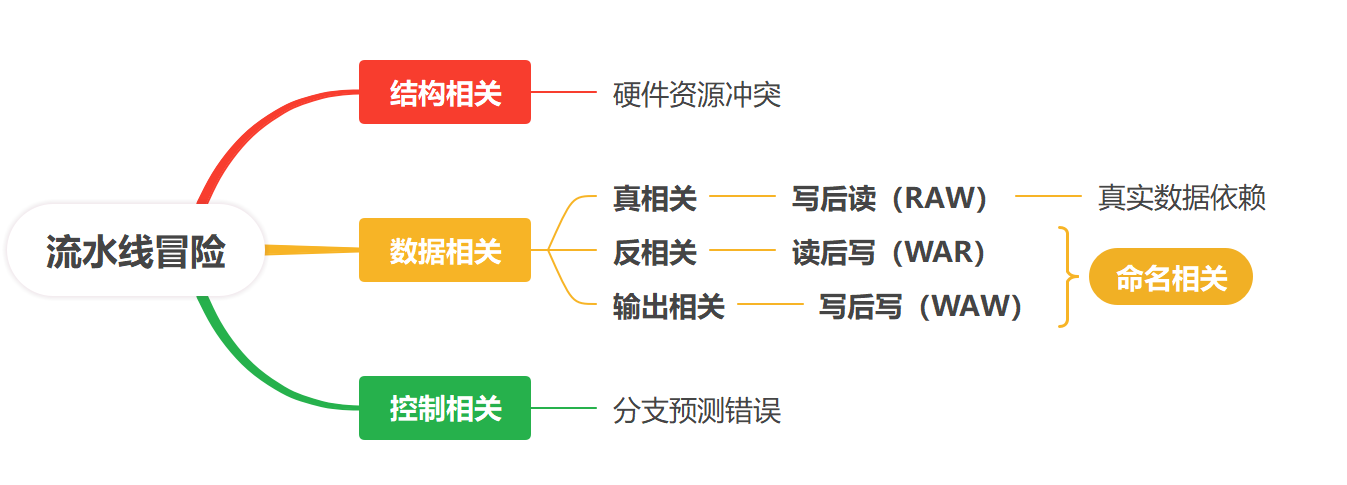
\includegraphics[width=10cm]{流水线冒险}
    \caption{流水线冒险概念图}\label{fig:pipeline-adventure}
\end{figure}

\begin{table}[htb]
    \begin{minipage}[t]{.32\textwidth}
        \centering
        \begin{tabular}{|cccc|}
        \hline
            \verb!ADD! & \textcolor{red}{$r_1$} & $r_2$ & $r_3$ \\
            \verb!ADD! & $r_4$ & \textcolor{red}{$r_1$} & $r_5$ \\
        \hline
        \end{tabular}
        \subcaption{真相关,写后读}
    \end{minipage}
    \begin{minipage}[t]{.32\textwidth}
        \centering
        \begin{tabular}{|cccc|}
        \hline
            \verb!ADD! & $r_4$ & \textcolor{red}{$r_1$} & $r_5$ \\
            \verb!ADD! & \textcolor{red}{$r_1$} & $r_2$ & $r_3$ \\
        \hline
        \end{tabular}
        \subcaption{反相关,读后写}
    \end{minipage}
    \begin{minipage}[t]{.32\textwidth}
        \centering
        \begin{tabular}{|cccc|}
        \hline
            \verb!ADD! & \textcolor{red}{$r_1$} & $r_2$ & $r_3$ \\
            \verb!ADD! & \textcolor{red}{$r_1$} & $r_2$ & $r_4$ \\
        \hline
        \end{tabular}
        \subcaption{输出相关,写后写}
    \end{minipage}
    \caption{数据相关的例子(注:\texttt{ADD} $r_i\ r_j\ r_k$ 表示 $[r_i]\gets [r_j]+[r_k]$)}\label{tab:instruction-hazard}
\end{table}

\subsection{静态流水线解决指令相关}

\textcolor{blue}{明确:在静态流水线中,指令不能乱序执行。}

\subsubsection{数据相关}
\begin{itemize}
    \item 数据相关包括 RAW、WAW、WAR,其中 WAW 和 WAR 属于命名相关,可以通过寄存器更名的方式解决。RAW 是真实数据依赖相关,需要用阻塞、前递等方法。
    \item 可以用 \Rare{阻塞} (stall)的方式解决数据相关。当相关指令在译码阶段发现与尚未执行完的指令存在数据相关,则阻塞在译码阶段,直到相关指令完成写回阶段。\textcolor{cyan}{\small (例如表 \ref{tab:instruction-hazard}(a) 种情况中,下方指令 \texttt{ADD}\ $r_4\ r_1\ r_5$ 需要读寄存器 $r_1$ 的值,那么它在取指阶段完成后会阻塞,直到上方指令 \texttt{ADD}\  $r_1\ r_2\ r_3$ 完成写回阶段后,才会继续译码阶段的执行。因此下方指令会在上方指令的执行、访存、写回阶段阻塞,共空 3 拍。参考 PPT 《Chapter09\_ 指令流水线-1.pptx》第 55 页。)}
    \item 可以用 \Rare{前递} (forwarding)的方式解决数据相关。当指令结果产生后(执行阶段或访存阶段完毕),立即将此结果送到后续相关指令的译码阶段中。
\end{itemize}

\subsubsection{控制相关}
\begin{itemize}
    \item 控制相关一般指跳转指令和取指 PC 指令的相关。解决控制相关主要有以下方法:
    \item 引入流水线阻塞法。如译码阶段遇到分支指令则暂停取指,或取消下一条指令的取回。
    \item \Rare{延迟槽}(delay slot)技术。设立一个延迟槽,存放条件分支指令的\textbf{紧接下一条}指令;不管条件分支指令是否跳转,都执行延迟槽中的指令。如果条件的确不满足,再取消延迟槽指令的执行。
    \item 转移预测。\textcolor{cyan}{(下文提到)}
    \item 循环展开。\textcolor{cyan}{(下文提到)}
\end{itemize}

\paragraph{异常处理}(了解)
\begin{itemize}
    \item 异常多种多样,在指令执行的任一阶段均可能发生。在指令内可恢复异常的处理比较困难。
\end{itemize}

\subsection{支线 [L09.2]·流水线的性能指标}
假设 $n$ 条指令,$k$ 段流水,每一段所用时间为 $\Delta t_i(i=1,2,\dots,k)$。
\begin{itemize}
    \item 流水线\Rare{瓶颈段}:指流水线耗时最长的一段。
    \item 流水线\Rare{吞吐率}:指单位时间内流水线完成的任务数量或输出的结果数量。
    \item \Epic{最大吞吐率} $TP_\mathrm{max}$:取决于流水线的瓶颈段所需时间,即
\begin{equation}\label{eq:TPmax}
    TP_\mathrm{max} = \dfrac{1}{\max\limits_{i}\{\Delta t_i\}}
\end{equation}
    \item \Legend{实际吞吐率} $TP$:等于指令条数 $n$ 与总时间 $T$ 之比:
\begin{equation}\label{eq:TP}
    TP = \dfrac{n}{T_\text{流水}} = \dfrac{n}{\sum_{i=1}^k \Delta t_i + (n-1)\cdot \max\limits_{i}\{\Delta t_i\}}
\end{equation}

    \item \Legend{流水线加速比} $S$:指同功能下非流水线的用时与流水线的用时之比:
\begin{equation}\label{eq:S}
    S = \dfrac{T_{\text{非流水}}}{T_{\text{流水}}} = \dfrac{n\cdot \sum_{i=1}^k \Delta t_i}{\sum_{i=1}^k \Delta t_i + (n-1)\cdot \max\limits_{i}\{\Delta t_i\}}
\end{equation}

    \item \Legend{流水线效率} $E$(或 $\eta$):指 $n$ 个任务占用的时空区与总时空区之比:
\begin{equation}\label{eq:E/eta}
\begin{split}
    E &= \dfrac{\text{有效时空区}}{\text{总时空区}} = \dfrac{n\cdot \sum_{i=1}^k \Delta t_i}{k\cdot T_\text{流水}} \\
    &= \dfrac{n\cdot \sum_{i=1}^k \Delta t_i}{k\cdot\left(\sum_{i=1}^k \Delta t_i + (n-1)\cdot \max\limits_{i}\{\Delta t_i\}\right)}
\end{split}
\end{equation}
\end{itemize}

\begin{subject}{专题·流水线时空图作图}
时空图有两种:
\begin{itemize}
    \item 一种是以横轴为时间、纵轴为流水段的时空图,在分析流水线的性能指标时,一般采用这一种。
    \item 另一种是以横轴为时间、纵轴为指令的时空图,在分析流水线的阻塞情况时,一般采用这一种。
\end{itemize}
对于前面一种流水线,在作图时应注意:
\begin{itemize}
    \item 有序作图,最好用直尺;
    \item 留意是\colorbox{teal!30}{静态流水线}还是\colorbox{teal!30}{动态流水线};
    \item 有的流水线只允许部分流水段并行,此时「瓶颈段」可能有变;
    \item 要留意数据冲突、控制冲突等带来的阻塞。
\end{itemize}
此外,通常吞吐率 $TP,TP_\mathrm{max}$ 含 $\Delta t$ 项,而加速比 $S$ 和效率 $E$ 不含 $\Delta t$ 项。

\end{subject}

\subsection{指令调度技术·循环展开}
\begin{itemize}
    \item 编译器(软件)的静态调度可以有效缓解控制相关。
    \item \Rare{循环展开}技术是静态调度的一种。它通过展开循环扩大基本块、移动不相关指令、寄存器重命名、巧妙设置偏移量等方法,将每次循环从 8 拍降低至 3.5 拍。
    \item 软件调度和硬件调度的区别:软件调度范围更大,而硬件调度可以掌握一些编译时不明确的相关性信息。
\end{itemize}

\section{(第9章)指令流水线·下}
\subsection{提高流水线效率·动态调度}

\begin{itemize}
    \item \Epic{动态调度}解决 \textbf{RAW,WAR,WAW 即数据相关} 问题,其基本思想是「乱序执行,乱序完成,有序提交」。
    \item CDC6600 \Rare{记分板算法} 是乱序执行,乱序完成,\textbf{乱序提交}的算法,并不能精确中断。
\end{itemize}

\subsubsection{Tomasulo 算法}
\begin{itemize}
    \item \Epic{Tomasulo 算法}(原始版)的基本思想仍是「乱序执行,乱序完成,\textbf{乱序提交}」,不能精确中断。
    \item Tomasulo 算法 的关键组件有:
    \begin{itemize}[itemsep=0pt,parsep=0pt]
        \item \Rare{保留站}:用来缓存源操作数,跟踪操作数是否就绪。
        \item 寄存器重命名:避免 WAR,WAW 阻塞\textcolor{cyan}{\small (要求能对 WAW,WAR 寄存器手工重命名)}
        \item 结果总线(CDB):用于广播指令完成的结果。
    \end{itemize}
    \item Tomasulo 算法的大致流程:指令发射 $\to$ 执行 $\to$ 写回。
\end{itemize}

\subsubsection{重排序缓存(ROB)}
\begin{itemize}
    \item \Epic{重排序缓存(ROB)}(reorder buffer)给 Tomasulo 算法打了一个「补丁」,这使得 ROB 加持下的 Tomasulo 算法获得了「乱序执行,乱序完成,\textbf{有序提交}」的能力,能够精确中断。
    \item ROB 在工作时,存储指令执行结果,直到确认无误后更新寄存器,释放 ROB 相应项数据。
    \item ROB+Tomasulo 算法的大致流程:指令发射 $\to$ 执行 $\to$ 写回 $\to$ 提交。
\end{itemize}

\subsection{提高流水线效率·多发射}
\subsubsection{支线 [L09.5]·多发射技术}
\begin{itemize}
    \item \Epic{多发射技术}(multiple issue):在每个时钟周期发射不止一条指令。
    \item 引入多发射技术后,变成「超标量」处理器、「超流水线」,一般采用动态流水线。设计开销更大。
    \item \Rare{IPC}:Instruction Per Cycle,即每一时钟周期发射的指令条数。目标为 $\mathrm{CPI}<1$ 或 $\mathrm{IPC} >1$ ,方法有:
    \begin{itemize}[itemsep=0pt,parsep=0pt]
        \item \Rare{超标量}:一次发射多条指令;
        \item \Rare{超长指令字(VLIM)}:把几条指令的操作组装成固定格式的长指令;
        \item 向量处理机:专用来计算矩阵、张量等多维数据。
    \end{itemize}
    其中\textbf{前两种方法}算作多发射技术。
\end{itemize}

\subsection{提高流水线效率·转移预测}
\begin{itemize}
    \item \Epic{转移预测}(也称转移猜测)技术解决\textbf{控制相关}问题。
    \item 转移预测在硬件上依靠「转移预测器」实现。转移预测器基于当前 PC 值和过去的转移历史记录,给出转移方向和目标地址。
    \item 下文提到的都是动态转移预测行为。
\end{itemize}

\subsubsection{转移历史表}
\begin{itemize}
    \item \Epic{转移历史表(BHT)}用 PC 低位作为索引,记录同一项上次转移是否成功。 BHT 有两个属性:多位PC、1 位转移结果。
    \item 两位 BHT 表方法:连续两回猜错才会改变猜测方向。其状态图如图 \ref{fig:2bit-BHT} 所示。
    \item 两位 BHT 表比一位 BHT 表更好,体现在循环间隙猜测更优。在每个循环间隙中(跳转方向记录中的 101 子段),一位 BHT 表会猜错 2 次,而两位 BHT 表仅猜错 1 次。
\end{itemize}

\begin{figure}[htb]
    \centering
    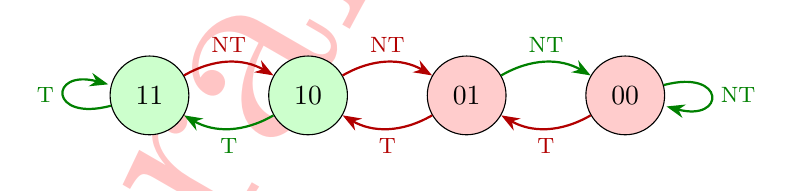
\begin{tikzpicture}[>=Stealth,
    node/.style={circle, minimum size=1cm, draw=black},
    wrong/.style={->, thick, red!70!black},
    correct/.style={->, thick, green!50!black}]
        \node (11) [node, fill=green!20] {11};
        \node (10) [node, right=of 11, fill=green!20] {10};
        \node (01) [node, right=of 10, fill=red!20] {01};
        \node (00) [node, right=of 01, fill=red!20] {00};
        \draw[wrong] (11) edge[bend left] node[font=\footnotesize, midway, above] {NT} (10);
        \draw[correct] (10) edge[bend left] node[font=\footnotesize, midway, below] {T} (11);
        \draw[wrong] (10) edge[bend left] node[font=\footnotesize, midway, above] {NT} (01);
        \draw[wrong] (01) edge[bend left] node[font=\footnotesize, midway, below] {T} (10);
        \draw[correct] (01) edge[bend left] node[font=\footnotesize, midway, above] {NT} (00);
        \draw[wrong] (00) edge[bend left] node[font=\footnotesize, midway, below] {T} (01);
        \draw[correct] (00) edge[loop right] node[font=\footnotesize, midway, right] {NT} (00);
        \draw[correct] (11) edge[loop left] node[font=\footnotesize, midway, left] {T} (11);
    \end{tikzpicture}
    \begin{tikzpicture}[>=Stealth, scale=0.7]
        \node (A) [circle, draw=black, fill=green!20, minimum size=0.5cm]  at (0,3) {};
        \node (B) [circle, draw=black, fill=red!20, minimum size=0.5cm]  at (0,2) {};
        \draw [->, thick, green!50!black] (-0.4,1) -- (0.4,1);
        \draw [->, thick, red!70!black] (-0.4,0) -- (0.4,0);
        \node [right, font=\small ]at (0.4, 3) {猜测跳转(T)};
        \node [right, font=\small] at (0.4, 2) {猜测不跳转(NT)};
        \node [right, font=\small] at (0.4, 1) {猜测正确};
        \node [right, font=\small] at (0.4, 0) {猜测错误};
    \end{tikzpicture}
    \caption{两位 BHT 状态图(箭头上标识为实际发生结果)}\label{fig:2bit-BHT}
\end{figure}

\begin{itemize}
    \item \Rare{分支目标缓冲(BTB)}:在跳转前,先对两种结果提前准备,未雨绸缪,失效时再替换。
    \item \Rare{相关分支预测}(correlated branch prediction):建立一个 $(m,n)$ 预测器,它考察此前的 $m$ 条分支记录(总共 $2^m$ 种可能性),建立 $n$ 位 BHT 表。特别地,$(0,2)$ 预测器即退化为两位 BHT 表。这样的 $(m,n)$ 预测器总共的位数为:$2^m\times n\times \text{涉及分支条目数}$。
    \item 组合分支预测器:类似机器学习中的「集成学习」思想,统合多个预测器的结果进行预测。
    \item \Rare{锦标赛预测法}:两个预测器互搏,任一预测器连续两次错误则换另一个。
\end{itemize}

\subsection{提高流水线效率·高速缓存}
\begin{itemize}
    \item \Rare{高速缓存}技术用于提升 RAW 数据冲突时的访存速度。
    \item 存储层次基本原理:\Rare{程序访问的局部性}。
\end{itemize}

\subsubsection{主存—Cache 层次}
\begin{itemize}
    \item Cache映像方式:直接映像、全相连、组相连;
    \item Cache失效替换:随机替换、先入先出(FIFO)、最近最少使用(LRU);
    \item Cache写命中时的策略:
    \begin{enumerate}[itemsep=0pt,parsep=0pt]
        \item \Epic{写回}(Write Back):写Cache时不写入主存,而当Cache数据被替换出去时才写回主存。优点是比较快;而缺点是实现相对复杂。
        \item \Epic{写穿透}(Write Through):写Cache时总是同时写入主存。优点是主存中的数据永远是最新的,实现容易;而缺点是比较慢。
    \end{enumerate}

    \item Cache 写失效时的策略:
    \begin{enumerate}[itemsep=0pt,parsep=0pt]
         \item \Rare{写分配}(Write Allocate):先把失效块读到Cache,再在Cache中写。常搭配「写回」法。
         \item \Rare{写不分配}(Write Non-allocate):直接将失效块写入主存。常搭配「写穿透」法。
    \end{enumerate}

    \item 有时会在「写穿透」的处理器和主存中设置一个\Rare{写缓冲}(Write Buffer),以平衡写入速度。
\end{itemize}

\subsubsection{Cache 性能分析与优化}
\begin{itemize}
    \item \Legend{平均访存时间(AMAT)}:指访存阶段的期望时间。若命中则取访问Cache时间(以时钟周期为单位);若不命中则外加惩罚时间乘以命中率,计算期望。AMAT 实际上就是访存指令的 CPI。
\begin{equation}\label{eq:AMAt}
    \mathrm{AMAT = HitTime + MissRate \times MissPenalty}
\end{equation}

\end{itemize}

\begin{subject}{专题·访存时间对计算机性能的影响}
如果将 CPU 计算时间划分为非访存指令时间(近似为ALU指令)和访存指令时间,那么公式 \eqref{eq:CPU-time} 中的 $CPI$ 可以稍稍扩展:
\begin{equation}\label{eq:CPU-time-AMAT}
    T_\mathrm{CPU} = I_N\times \left(\dfrac{I_{N\mathrm{ALU}} }{ I_N}\times CPI_{\mathrm{ALU}} + \dfrac{I_{N\mathrm{MEM}}}{I_N}\times AMAT\right)\times T_\mathrm{c}
\end{equation}
其中 $I_{N\mathrm{ALU}}$ 和 $I_{N\mathrm{MEM}}$ 分别为ALU指令和访存指令的条数,$I_N$ 为总指令条数,$T_\mathrm{c}$ 为时钟周期。

\begin{equation}\label{eq:CPU-time_AMAT-2}
    T_\mathrm{CPU} = I_N\times \left(CPI_\mathrm{exe} + \text{MemPerInst} \times \text{MissRate} \times \text{MissPenalty}\right)\times T_\mathrm{c}
\end{equation}
其中 MemPerInst 为每条指令的平均访存次数。
\end{subject}

\subsubsection{Cache失效原因与解决}
\begin{itemize}
    \item \Epic{Cache 失效原因(3C/4C)}:
    \begin{enumerate}
        \item \Rare{冷启动失效} (Cold/Compulsory Miss):第一次访问时的失效
        \item \Rare{容量失效} (Capacity Miss):因容量有限而被替换的失效
        \item \Rare{冲突失效} (Conflict Miss):不同主存行映射到同一Cache块的失效
        \item \Rare{一致性失效} (Coherence Miss):维护「Cache一致性」导致的失效
    \end{enumerate}
    
    \item 不同方法降低失效率(Miss Rate):
    \begin{enumerate}
        \item 增加块大小(但保持Cache容量不变):减少冷启动失效,但增加容量失效、冲突失效、失效惩罚; 
        \item 增加Cache容量:减少容量失效,增加访问时间;
        \item 增加相连度、「路猜测」和「伪相连」法:减少冲突失效;
        \item 软件优化(数组合并、循环交换、循环合并、数组分块等):综合降低失效率
    \end{enumerate}

    \item 降低失效惩罚(Miss Penalty)的方法:优先处理读失效、关键字优先、写合并、牺牲缓存(Victim Cache)、二级Cache等。

    \item 降低命中时间(Hit Time)的方法:简化Cache设计、增加Cache访问流水级、提高Cache访问并行性。
\end{itemize}

\subsection{支线 [L09.6]·I/O处理与存储系统}
\begin{itemize}
    \item \Rare{南北桥}:
    \begin{enumerate}[itemsep=0pt,parsep=0pt]
         \item 北桥快,连接CPU,连接内存,连接GPU;
         \item 南桥慢,连接I/O。
    \end{enumerate}

    \item 反映存储外设可靠性能的参数:
    \begin{enumerate}[itemsep=0pt,parsep=0pt]
         \item 系统可靠性(Reliability),用MTTF衡量;
         \item 系统可用性(Availability),用 $\mathrm{\frac{MTTF}{MTBF}}$ 衡量;
         \item 系统可信性(Dependability),不可度量。
         \item \Rare{平均无故障时间(MTTF)};
         \item \Rare{平均故障间隔时间(MTBF)} $\mathrm{= MTTF + MTTR}$;
         \item \Rare{平均修复时间(MTTR)}。
    \end{enumerate}

    \item 「廉价磁盘冗余阵列(RAID)」提高了系统可用性。
\end{itemize}


\section{(第10章)并行编程基础}
\subsection{三种并行行为}
\begin{itemize}
    \item \Rare{指令级并行(ILP)}:不相关的指令可以并行执行
    \item \Rare{数据级并行(DLP)}:对多个元素同时执行相同操作
    \item \Rare{任务/线程级并行(TLP)}:将不同任务(进程/线程)分布到不同处理单元并行执行
\end{itemize}

开发指令级并行的两种方法是:
\begin{enumerate}
    \item \textbf{基于硬件的动态开发方法}:也就是《指令流水线·下》介绍的四种方法:动态调度、多发射、转移预测、高速缓存。
    \item \textbf{基于软件的静态开发方法}:依赖于编译器在编译时对程序的分析与优化,例如循环展开。
\end{enumerate}

\subsection{Flynn分类法}
\begin{itemize}
    \item \Epic{Flynn 分类法}:根据\textbf{指令流}和\textbf{数据流}的多倍性对计算机系统结构进行分类。目前分成三种:
    \begin{enumerate}[itemsep=0pt,parsep=0pt]
        \item \Rare{单指令流单数据流(SISD)}
        \item \Rare{单指令流多数据流(SIMD)}
        \item \Rare{多指令流多数据流(MIMD)}
    \end{enumerate}

    \item 对于 MIMD 系统,还能按照信息传递方法分成:
    \begin{enumerate}[itemsep=0pt,parsep=0pt]
        \item 多处理机系统:基于共享存储器(Shared Memory)
        \item 多计算机系统:基于消息传递(Message Passing)
    \end{enumerate}
    其中内存组织方式还能细分为
    \begin{enumerate}[itemsep=0pt,parsep=0pt]
        \item 中心化内存(Global/Centralized Memory)
        \item 分布式内存(Distributed Memory)
    \end{enumerate}

    \item 因此还有一种 \Epic{Johnson 分类法},对 MIMD 系统进行分类:
    \begin{enumerate}[itemsep=0pt,parsep=0pt]
        \item 中心化内存+共享存储器(GMSV)
        \item 分布式内存+共享存储器(DMSV)
        \item 分布式内存+消息传递(DMMP)
    \end{enumerate}
\end{itemize}

\subsection{典型并行计算机结构与并行编程}
\begin{itemize}
    \item 典型并行计算机结构:
    \begin{enumerate}[itemsep=0pt,parsep=0pt]
        \item 对称多处理机(SMP)
        \item 工作站机群(COW)
        \item 大规模并行处理机(MPP)
    \end{enumerate}

    \item 典型并行编程环境:
    \begin{enumerate}[itemsep=0pt,parsep=0pt]
        \item SIMD数据并行编程
        \item \Rare{POSIX Threads 标准},简称 Pthread,IEEE官方标准
        \item \Rare{OpenMP} 共享存储编程标准
        \item \Rare{MPI} 标准
    \end{enumerate}

    \item 「并行编程的挑战」——联系第一章 Amdahl 定律计算和 CPI 计算
\end{itemize}

\section{多核处理器}

多核处理器可以这么分类:异构、同构;通用、专用;重核、轻核;多核、众核……要求通用多核处理器访存带宽和峰值性能差距不能太大。

\subsection{分支[L11.1]·单处理器时代的终结}
\begin{itemize}
    \item 单核处理器性能提升的瓶颈:频率墙、功耗墙、存储墙、应用墙。传统性能提升手段失效(如流水线、超标量等),主频增长停滞。
    \item 多核处理器成为必然趋势。
    \item 「新摩尔定律」:性能提升由「更快」转为「更宽」。多核(TLP)与数据级并行(DLP)将成为未来主流。
    \item FPGA优势、RAMP并行计算研究项目。
\end{itemize}

\subsection{分支[L11.2]·同时多线程}
\begin{itemize}
     \item \Rare{多线程}:在一个处理器上运行多个线程。
     \item 多线程的分类,如图 \ref{fig:multithread} 所示:
     \begin{enumerate}
        \item \Rare{细粒度}:线程切换于每条指令之间。采用「轮叫调度」。
        \item \Rare{粗粒度}:线程切换于代价高、时间长的阻塞出现之时。
     \end{enumerate}
     \item \Epic{同时多线程(SMT)}:是一种在多流出、动态调度处理器上同时开发线程级并行(TLP)和指令级并行(ILP)的改进的多线程技术。
     \item 换言之,同时多线程允许\textbf{单个}物理CPU核心同时执行\textbf{多个}线程的指令。通过共享执行资源(如ALU、寄存器等)实现。它只有在细粒度实现方式下才有意义。
\end{itemize}

\begin{figure}[htb]
  \centering
  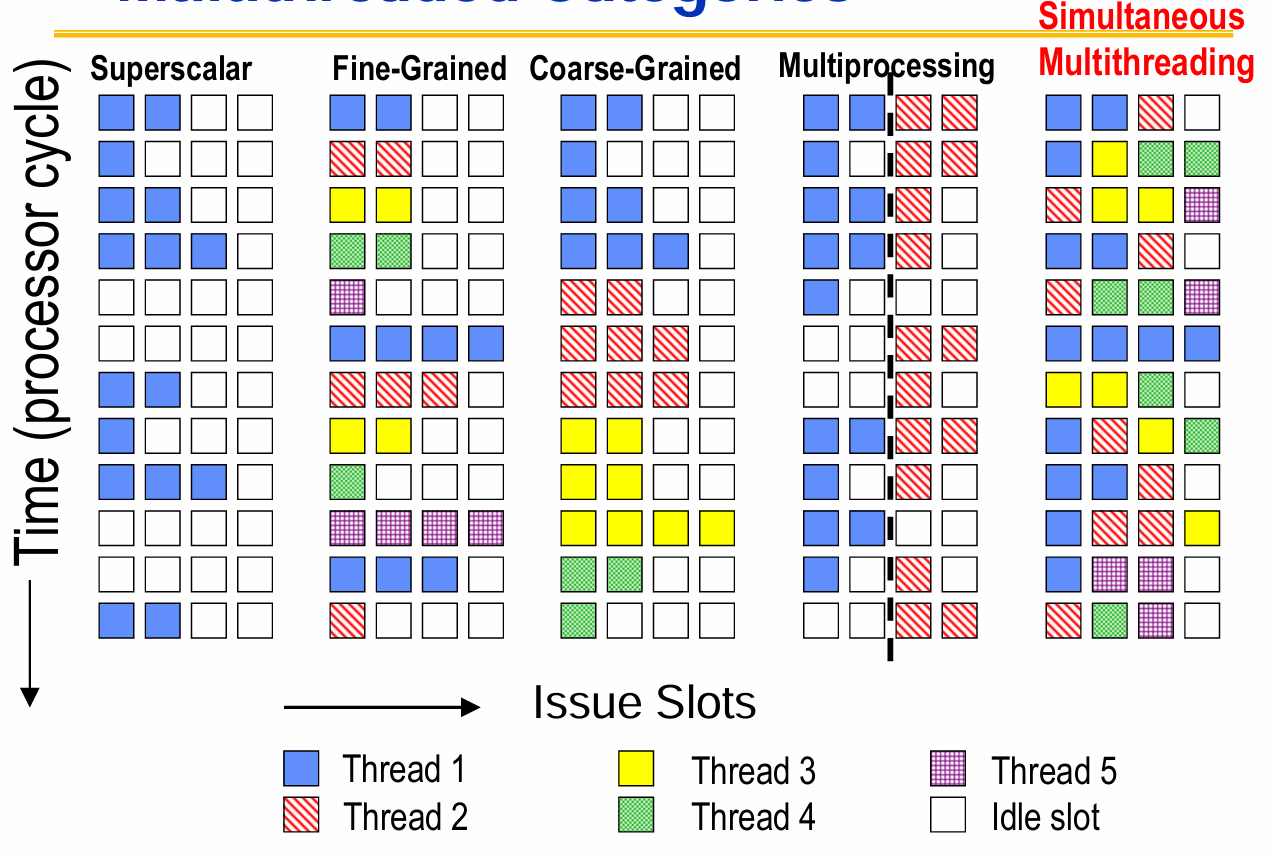
\includegraphics[width=10cm]{多线程分类.png}
  \caption{多线程分类(从左到右依次为超标量、细粒度、粗粒度、多处理器、同时多线程)}\label{fig:multithread}
\end{figure}


\subsection{访存结构、存储一致性模型}
\begin{itemize}
    \item 通用多核CPU的\Rare{片上Cache结构}:片内共享最后一级Cache(Last Level Cache,LLC),其他级别的Cache由片内私有,片间共享内存。
    \item 共享LLC结构细分为:集中式共享(UCA)、分布式共享(NUCA)。
    \item \Epic{存储一致性模型}:
    \begin{enumerate}
        \item \Rare{顺序一致性}:并行执行结果应等于多进程环境下的一个执行结果。\footnote{这类似于《数据库系统原理》中的「可串行化调度」:多个事务的并发执行是正确的,当且仅当其结果与按某一次序串行地执行这些事务时的结果相同。}
        \item \Rare{处理器一致性}:在任一取数操作 LOAD 允许被执行之前,所有在同一处理器中先于这一 LOAD 的取数操作都已完成;在任一存数操作 STORE 允许被执行之前,所有在同一处理器中先于这一 STORE 的访存操作(包括LOAD和STORE)都已完成。
        \item \Rare{弱一致性}:只在需要同步的同步点维护一致性。
        \item \Rare{释放一致性}:把同步操作细分为获取和释放操作。
    \end{enumerate}
    \item \Epic{Cache 一致性协议}:在多处理器系统中,同一个内存地址在不同Cache中的数据副本保持一致。有两种策略用于维护Cache一致性:
    \begin{enumerate}
        \item \Rare{写使无效}(Write Invalidate):当某处理器对共享数据进行写操作时,将其他Cache中的该数据副本标记为无效,后续其他处理器需重新读取最新值。
        \item \Rare{写更新}(Write Update):当某处理器修改共享数据时,立即将更新后的值广播到所有持有该数据副本的Cache,保持多副本一致。
    \end{enumerate}
    \item 写使无效和写更新是为了解决「如何传播新值」的问题。「侦听协议」和「目录协议」是为了解决「新值传播给谁」的问题。
\end{itemize}

\subsection{互连结构、同步机制}
\begin{itemize}
    \item \Rare{片上互联网络(NOC)}是一种典型的互联结构。它具有片上总线、交叉开关、拓扑结构、路由算法、路由表、流量控制等计算机网络都有的机制。
    \item \Rare{同步机制}:三种常见同步机制:
    \begin{enumerate}[itemsep=0pt,parsep=0pt]
        \item 互斥锁操作
        \item 路障操作
        \item 事务内存
    \end{enumerate}
    对于上述机制,有三种常见实现方式:读—改—写指令、LL/SC指令、用户级软件例程。
\end{itemize}

\newpage

\printindex
\backgroundsetup{contents=
\includegraphics{下半示例.png}, center, scale=1, angle=0, opacity=1}
\BgThispage

\end{document} 